In der Arbeitsgruppe LARISSA\footnote{\textbf{La}ser \textbf{R}esonance
\textbf{I}onisation \textbf{S}pektroscopy for \textbf{S}elective Tracer
\textbf{A}nalysis} des Instituts für Physik an der Johannes Gutenberg
Universität Mainz wurden über viele Jahre hinweg Methoden zur
Resonanzionisations-Massenspektrometrie (RIMS) entwickelt und verbessert.
Mithilfe dieser wurden in der Vergangenheit empfindliche und selektive
Ultraspurenbestimmungen einiger Elemente der seltenen Erden und der
Übergangsmetalle durchgeführt. Aber auch an Elementen aus den Reihen der
Lanthanoide und Actinoide wurden diese Methoden demonstriert. Vorraussetzung für
die Ultraspurenanalyse ist die hohe Isotopen- und Isobarenselektivität, welche
durch Kombination von elementselektiver resonanter Laserionisation und
isotopenselektiver Quadrupolmassenspektrometrie (QMS) realisiert wird.
Zur Laserionisation werden in Mainz zwei verschiedene Lasersysteme verwendet, bestehend zum einen
aus gepulst betriebenen Titan:Saphire-Lasern und zum anderen aus
Dauerstrich-Diodenlasern.\par
Ein wichtiges Teilgebiet dieser Untersuchungen beschränkt sich auf die
hochauflösende Ultraspurenanalyse von Uranisotopen (siehe Nuklidkartenausschnitt Abb.
\ref{fig:uran_nuklidkarte}) mittels HR-RIMS\footnote{\textbf{H}igh
\textbf{R}esolution-RIMS}.
\begin{figure}[h]
 	\centering
 	\fbox{\parbox{\dimexpr \linewidth - 2\fboxrule - 2\fboxsep}{
 	\centering
	    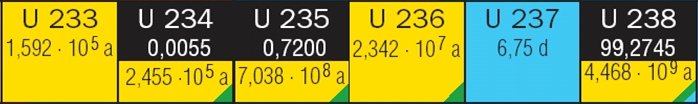
\includegraphics[width=\textwidth-5cm]{gfx/uran_nuklidkarte}
	}}
	\caption[Gesamter experimenteller Aufbau,
	schematisch]{Ausschnitt der Karlsruher Nuklidkarte für langlebige
	Uranisotope \cite{nuklidkarte}}\label{fig:uran_nuklidkarte}
\end{figure}
Das Schwermetall Uran ist das schwerste natürliche Element auf der Erde und
findet sich in den stabilen Isotopen $^{238}$U und $^{235}$U wieder, welche aus
Supernovea-Explosionen stammen. Das dritte stabile Isotop $^{234}$U
resultiert aus $\alpha$-$2\beta$-Zerfällen von $^{238}$U. Da $^{238}$U und
$^{235}$U aus keinen anderen Elementen nachgebildet werden können, lassen sich
aus dem durch die Lebenszeiten ermittelbaren natürlichen Isotopenverhältnis
$\nicefrac{^{235}\text{U}}{^{238}\text{U}}=0,00725$ Rückschlüsse auf die
Entstehungszeit unseres Sonnensystems ziehen. Das Isotop $^{236}$U entsteht
durch Einfang thermischer Neutronen aus $^{235}$U.
Verhältnisse $\nicefrac{^{236}\text{U}}{^{238}\text{U}}$ von $10^{-14}$ bzw.
$10^{-11}$ -- $10^{-9}$ resultieren im natürlichen Gleichgewicht aus
Neutronenflüssen der kosmischen Strahlung bzw. in Uranerzen \cite{Richter19999}.
Da in Kernreaktoren sehr hohe Neutronenflüsse herrschen, können dort
wesentlich höhere
$\nicefrac{^{236}\text{U}}{^{238}\text{U}}$-Isotopenverhältnisse von
$1,4\cdot10^{-4}$ bis $2,4\cdot10^{-4}$ erzielt werden. Das natürliche Verhältnis kann also als Referenz dienen, um einen anthropogenen Eintrag von Uran in die Umwelt
nachzuweisen.\par
Die große Wichtigkeit dieses Nachweises ist in der Tatsache
begründet, dass die Aufnahme von erhöhten Mengen Uran durch den Körper toxisch
wirkt und durch die kurzlebigen Uranisotope eine erhöhte Strahlenbelastung
gegeben ist. Die Obergrenze für die unbedenkliche Aufnahmerate von Uran liegt
bei $0,6\,\text{\textmu g}$ pro Tag und kg Körpergewicht, wobei das Grund- bzw.
Trinkwasser mit $10^{-6}\,\nicefrac{\text{g}}{\text{l}}$ belastet ist
\cite{who:2005}. Die Überhöhungen der natürlichen Verhältnisse von 
$\nicefrac{^{236}\text{U}}{^{238}\text{U}}$ resultieren maßgeblich aus
Nuklearwaffentests bis einschließlich 1998 und nicht zuletzt aus Reaktorunfällen
wie der bekannte "`Tschernobyl-Unfall"' oder der aktuell brisante Unfall in
Fukushima, Japan. Da die Kontamination der Umwelt großflächig verteilt sein
kann, ist es notwendig, sehr kleine Isotopenverhältnisse messen zu können. Die
HR-RIMS bietet hierfür hervorragende Möglichkeiten.\par
Um mithilfe von Lasern nicht nur elementselektiv, sondern auch
isotopenselektiv ionisieren zu können\footnote{Isotopieverschiebung, siehe
\ref{subsec:isotopieverschiebung}} und hochauflösende Spektroskopie zu
betreiben, wird sehr schmalbandiges Laserlicht benötigt, welches mit
Dauerstrichlasern erzeugt werden kann. Diodenlaser sind für diesen Einsatz eine
optimale und kostengünstige Lösung. Da die Übergangslinien bei Benutzung von
schmalbandigen Diodenlasern teilweise ebenfalls nur wenige MHz schmal sind, ist
eine aktive Frequenzstabilisierung der Laser unabdingbar.\par
Im Rahmen dieser Diplomarbeit soll ein frequenzstabilisiertes Diodenlasersystem
entwickelt und für den Einsatz zur HR-RIMS an Uran charakterisiert werden.
Folgende Anforderungen werden an das Lasersystem und die Stabilisierung gestellt:
\begin{setlength}{\leftmargini}{1cm}
	\begin{description}
		\item[Stabilität und Frequenzsicherheit]\hfill\\
			Die Laser sollen sowohl auf langen als auch kurzen Zeitskalen (wenige ms bis
			einige Stunden) stabil auf ihrer Frequenz gehalten werden. Die
			Kurzzeitstabilität wird gefordert, um laserinduzierte Zählratenfluktuationen
			zu minimieren. Dabei sind Frequenzfluktuationen von deutlich weniger als
			$10\,$MHz angestrebt. Langzeitdrifts sollen völlig eliminiert werden, um auch
			über lange Zeiten angelegte Messungen reproduzierbar zu machen. Dabei ist es
			wichtig, dass die Stabilisierung ausfallsicher implementiert wird, was
			fehlerfreie Relativfrequenzdetektion und präzise Steuerung der Laser
			vorraussetzt.
		\item[gezielte Frequenzverstimmung]\hfill\\
			Um gezielt atomare Übergangsfrequenzen anfahren und spektroskopische
			Messungen durchführen zu können, soll die Möglichkeit der individuellen
			Laserfrequenzverstimmung implementiert werden. Insbesondere bei
			Isotopenverhältnismessungen ist ein regelmäßiger Wechsel der
			Anregungsschritte verschiedener Uranisotope notwendig.
		\item[Geschwindigkeit]\hfill\\
			Zur Steigerung der Messeffizienz wird angestrebt, Frequenzverstimmungen
			möglichst schnell abzuwickeln. Frequenzverstimmungen von einigen
			GHz sollen innerhalb weniger Sekunden vollzogen werden, was gerade bei
			Isotopenverhältnismessungen von großem Vorteil sein kann.
		\item[Automatisierung]\hfill\\
			Um Messungen präzise, systematisch und ohne großen Aufwand durchführen zu
			können, soll die Steuerung der Laser - soweit möglich - vollständig
			automatisiert werden, wobei als Schnittstelle zum Experimentator ein PC mit
			einem \textit{Labview}-Programm dienen soll. Neben der Laserkontrolle soll
			auch die Messdatenaufnahme über denselben PC erfolgen.
	\end{description}
\end{setlength} 
Zur Realisierung der Laserstabilisierung wird die bewährte Methode des
\textit{Fringe-Offset-Locking} \cite{kuschnick:2000:diplomarbeit}, basierend auf
einem \textit{scanning FPI}\footnote{\textit{scanning FPI}: ein in der Länge
verstimmbares Fabry-Pérot-Interferometer}, durch eine kommerzielle
Stabilisierungstechnik, basierend auf einem festen Quadraturinterferometer,
ergänzt.\par
Der Inhalt dieser Arbeit soll die Entwicklung und den Aufbau des Lasersystems,
der optischen Komponenten der Frequenzstabilisierung inklusive Elektronik, die
Programmierung der Software zur Stabilisierung und Experimentsteuerung und die
Charakterisierung des Gesamtsystems umfassen.
